\documentclass[a4paper]{article}
\usepackage{amsfonts}
\usepackage{amsmath}
\usepackage{amssymb}
\usepackage{graphicx}
\usepackage{float}

\begin{document}

\noindent \large Auteur: Siebe Haché \\
\noindent \large Studierichting: Informatica \\
\noindent \large Oefeningenreeks 3H nr. 12.9 \\
\medskip
\normalsize

Bestudeer de functie met de volgende poolvergelijking:\\

$ r = 1 + \sin^4 3\theta$\\

De functie is gedefinieerd voor alle $\theta \in \mathbb{R}$\\

periode:\\

van $\sin 3\theta$ is $\dfrac{2\pi}{3}$. Omdat de macht even is herhaalt de functie zich elke $\dfrac{\pi}{3}$.\\

Nulpunten:\\

$r = 0 \Leftrightarrow 1 + \sin^4 3\theta = 0 \Leftrightarrow \sin^4 3\theta = -1$. \\

Dit heeft geen reële oplossingen, dus ($r \ge 1$). \\

Onderzoek eetrste afgeleide: \\

$r' = 4\sin^3 3\theta \cdot (\cos 3\theta \cdot 3) = 12 \sin^3 3\theta \cos 3\theta$ \\

$r' = 0 \Leftrightarrow \sin 3\theta = 0$ of $\cos 3\theta = 0$ \\

$3\theta = k\pi \Rightarrow \theta = \dfrac{k\pi}{3}$ \\

$3\theta = \dfrac{\pi}{2} + k\pi \Rightarrow \theta = \dfrac{\pi}{6} + \dfrac{k\pi}{3}$ \\

In $[0, \pi]$ zijn de punten: $\theta \in \left\{0, \dfrac{\pi}{6}, \dfrac{\pi}{3}, \dfrac{\pi}{2}, \dfrac{2\pi}{3}, \dfrac{5\pi}{6}, \pi\right\}$. \\

\begin{tabular}{c|cccccccc}
 $\theta$ & $0$    &            & $\dfrac{\pi}{6}$ &            & $\dfrac{\pi}{3}$ &            & $\dfrac{\pi}{2}$ &  \\ \hline
 $r$      & $1$    & $+$        & $2$              & $+$        & $1$              & $+$        & $2$              & $+$ \\
 $r'$     & $0$    & $+$        & $0$              & $-$        & $0$              & $+$        & $0$              & $-$  \\ \hline
 $r$      & $m(1)$ & $\nearrow$ & $M(2)$           & $\searrow$ & $m(1)$           & $\nearrow$ & $M(2)$           & $\searrow$  \\
\end{tabular} \\


grafiek:\\

\begin{figure}[H]
    \centering
    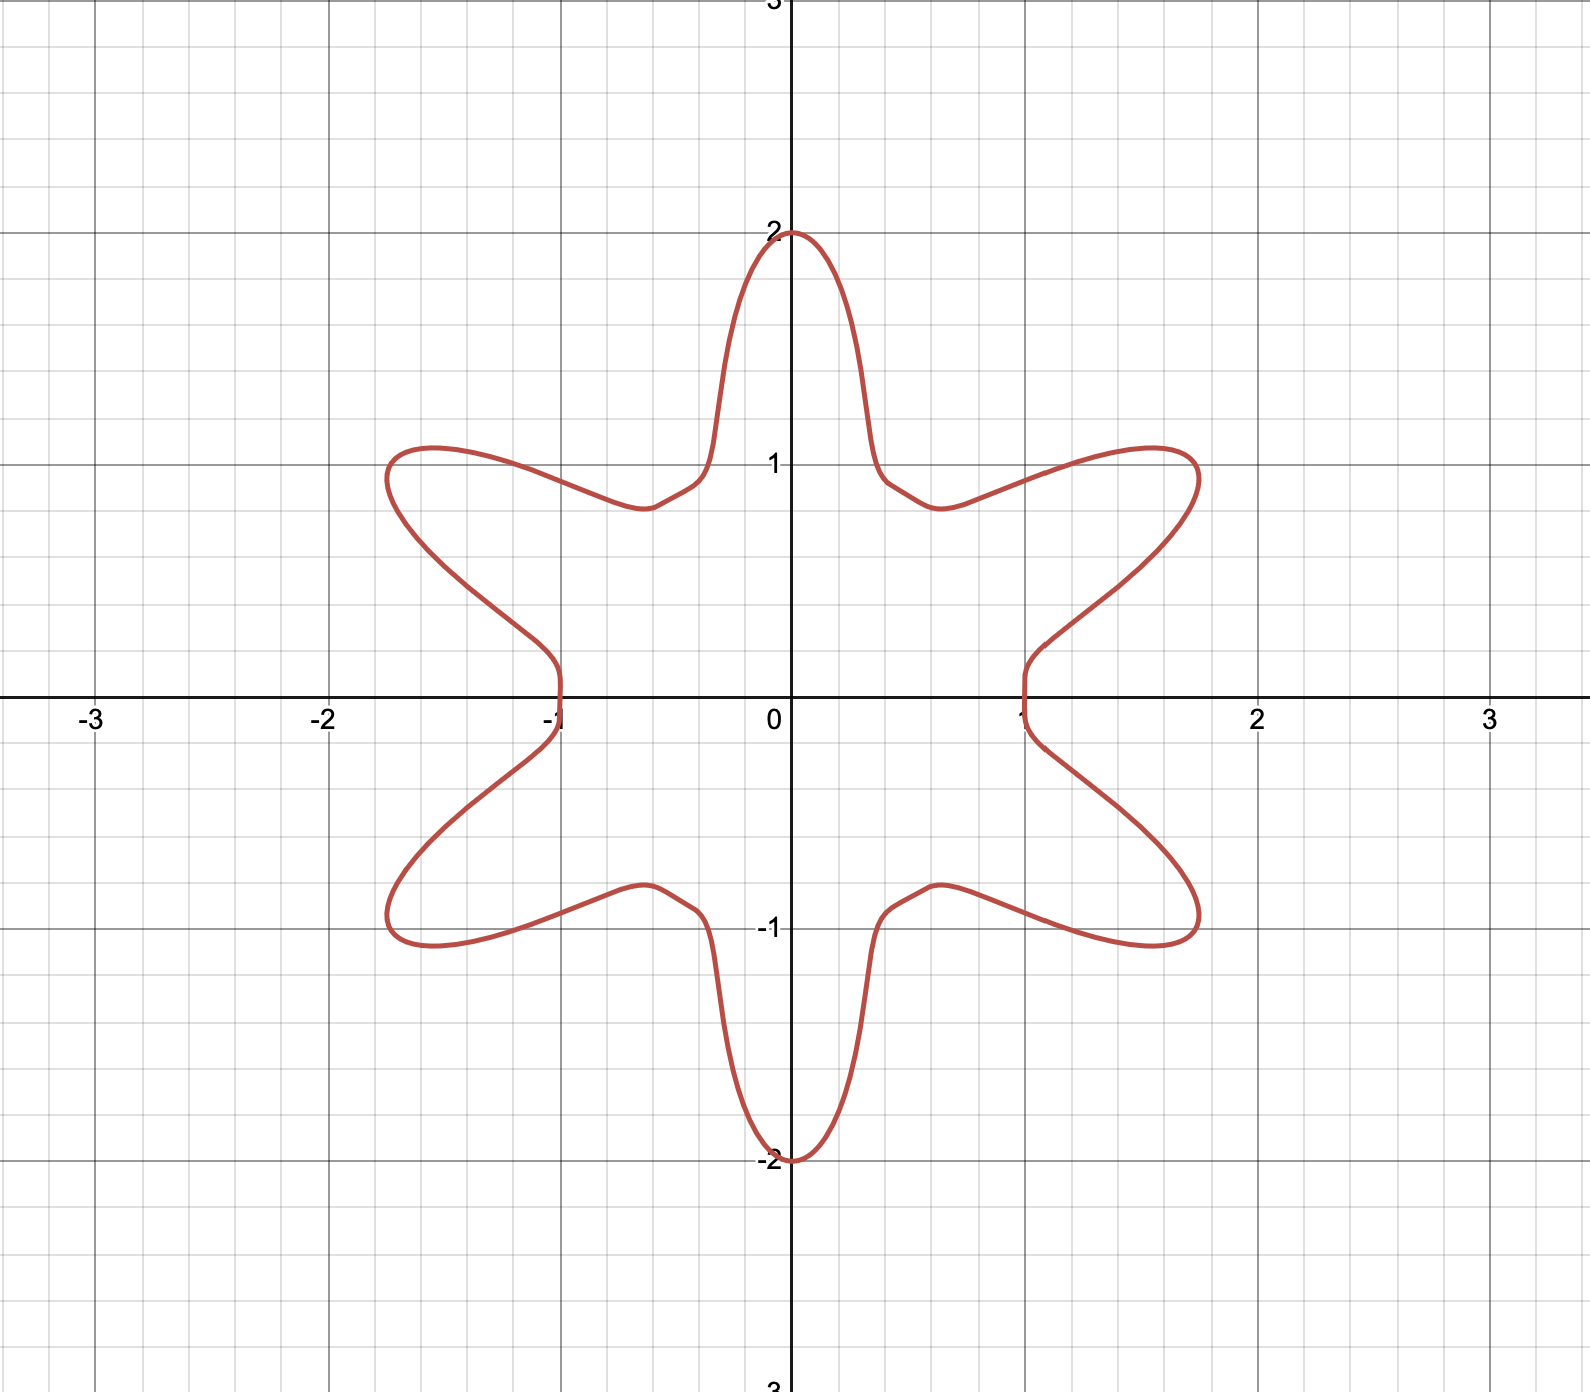
\includegraphics[width=0.6\textwidth]{3H-12.9-siebe.hache.INF.png}
\end{figure}

\begin{thebibliography}{999}
\bibitem{a} Grafiek gemaakt met Desmos.com
\end{thebibliography}

\end{document}